% Extensionly - análise e projeto de software, artefatos da implementação, maior capítulo de todos, modelo de domínio, diagrama de componentes, paradigma de programação, tecnologias, processo da engenharia de software, separação frontend/backend (com mais detalhes técnicos), usar figuras e modelos
%==============================================================================
\chapter{Extensionly Backend Design}\label{extensionly}
%==============================================================================

% ===================================
% Este capítulo descreve particularidades da ferramenta Extensionly, decisões relacionadas ao backend entre outras decisões de design.

This chapter describes the particularities of the Extensionly tool, decisions related to the backend and other design decisions.
% ===================================

\section{Initial Considerations}\label{sec:ext-considerations}
% ===================================
% A ferramenta Extensionly, por ter como objetivo incorporar e reproduzir todos ou a maioria dos processos envolvendo atividades de extensão, o seu desenvolvimento é divido entre dois alunos estando um responável pelo frontend e outro pelo backend que é o objetivo deste trabalho. 
% Para o desenvolvimento acontecer de forma fluida e performatica, a comunicação entre os desenvolvedores deve ser constante, pois qualquer mudanca em regras de negocio devem estar muito claras por ambas as partes.

The Extensionly tool, as it aims to incorporate and reproduce all or most of the processes involving \acl{OA}, its development is divided between two students, one being responsible for the frontend and the other for the backend, which is the objective of this work.
The project will be versioned utilizing Git, a version control tool designed to efficiently and quickly manage any project, no matter how big or small \cite{chacon2014pro}. The source code will be split between two repositories, one for the frontend\footnote{Extensionly Frontend code is available at \url{https://github.com/Dalepfell/extensionly-frontend}} and one for the backend\footnote{Extensionly Backend code is available at \url{https://github.com/IgorDalepiane/extensionly-backend-service}}.

For development to happen in a fluid and performative way, communication between developers must be constant, as any change in business rules must be very clear by both parties.
% ===================================

% ===================================
% O propósito geral da ferramenta além de suportar variados processos envolvendo extensão universitária, é estreitar as relações entre a comunidade externa e acadêmica, criando um canal de comunicação em que possa ser geradas demandas para a universidade. 
% Sendo assim, os alunos vão estar cada vez mais acostumados e vinculados com a comunidade como um todo, atribuindo muito valor e experiencia a sua formação.

The general purpose of the tool, in addition to supporting various processes involving university outreach, is to strengthen relations between the external and academic community, creating a communication channel in which demands can be generated for the university.
Therefore, students will be increasingly accustomed to and linked to the community as a whole, attributing much value and experience to their formation.
% ===================================

% ===================================
% A ferramenta tem como primeiro objetivo ser utilizada pela unipampa campus alegrete, mas não dispensando possiveis expansões futuras, para todos os campus da instituição e até mesmo para outras instituições do Brasil. 
% Para isto a implementação deve ser realizada de uma maneira que seja diminuido o custo quando estas novas decisões de projeto forem tomadas.

The first objective of the tool is to be used by \ac{UNIPAMPA} Campus Alegrete, but not dispensing with possible future expansions, for all the institution's campuses and even for other institutions in Brazil.
For this the implementation must be carried out in a way that the cost is reduced when these new design decisions are made.
% ===================================
% Ferramenta Desenvolvida em conjunto
% Comunicação entre os dois
% Proposito da ferramenta é estreitar as relações entre a comunidade, alunos estrem mais vinculados com a comunidade como um todo,
% Objetivo de fazer um teste piloto em 2023 janeiro
% Primeiro case da ferramenta é a Unipampa, mas ja pensando em possiveis expansoes para todas as instituições

\section{Extensionly Requirements}\label{sec:ext-req}
% ===================================
% Esta seção esta direcionada a apresentar em mais detalhes os requisitos funcionais levantados pelo estudo, o qual foi divido em duas partes principais, primeiro sendo conduzida uma revisão na literatura cinza, como apresentado na \Cref{grey_literature}, e depois com os resultados analisados e transformados em estorias de usuario, foi aplicado o survey descrito na \Cref{sec:5} 
This section is intended to present in more detail the functional requirements raised by the study, which was divided into two main parts, first being conducted a review of the gray literature, as presented in \Cref{grey_literature}, and then, with the results analyzed and transformed into user stories, they were applied to the survey described in \Cref{sec:5}

% ===================================

\subsection{Requirements Obtained through the Grey Literature Review}\label{req-grey}
% ===================================
% Na execução da revisão da literatura cinza, analisando outras ferramentas similares, como ja bem descrito na \Cref{grey_literature}, foram levantados algumas funcionalidades presentes nas ferramentas como mostra a \Cref{sec:gl-feature-matrix}, dentre eles 28 (twenty eight) \acp{FR} foram selecionados para participarem da proxima fase, o survey. 
% Então os desenvolvedores junto com seu supervisor, analisaram caso a caso e classificaram a sua prioridade entre:
% \begin{inparaenum}[(1)]
% \item High 
% \item Medium 
% \item Low 
% \end{inparaenum}.
% Alguns destes requisitos foram removidos após a classificação, pois eram muito complexos para o contexto de um \ac{MVP}, ou não faziam parte de escopo simplesmente.

In carrying out the review of the gray literature, analyzing other similar tools, as already described in \Cref{grey_literature}, some functionalities present in the tools were raised, as shown in \Cref{sec:gl-feature-matrix}, among them 28 (twenty eight) \acp{FR} were selected to participate in the next phase, the survey.
So the developers, together with their supervisor, analyzed it on a case-by-case basis and ranked their priority among:
\begin{inparaenum}[(1)]
    \item High;
    \item Medium;
    \item Low.
\end{inparaenum}
Some of these requirements were removed after classification, as they were too complex for the context of an \ac{MVP}, or simply not in scope. All the initial requirements among with their priority can be found in \Cref{tab:initial-requirements}.
% ===================================

\begin{table}[!htb]
  \centering
  \setlength{\aboverulesep}{0pt}
  \setlength{\belowrulesep}{0pt}
  \caption{Initial Requirements}
  \label{tab:initial-requirements}
  \footnotesize
  \begin{tabular}{c|l|c}
    \toprule
    \rowcolor[rgb]{0.753,0.753,0.753} \textbf{ID} & \multicolumn{1}{c|}{\textbf{Requirement}}                    & \textbf{Priority} \\
    \hline
    \rowcolor[rgb]{0.898,0.898,0.898} FR. 01      & Propose new OAs                                              & High              \\
    FR. 02                                        & Allow enrollments in OA                                      & High              \\
    \rowcolor[rgb]{0.898,0.898,0.898} FR. 03      & Record participant attendance                                & High              \\
    FR. 04                                        & Review and approve OA proposals                              & High              \\
    \rowcolor[rgb]{0.898,0.898,0.898} FR. 05      & Text search for OAs                                          & High              \\
    FR. 06                                        & Registration of OA prerequisites                             & High              \\
    \rowcolor[rgb]{0.898,0.898,0.898} FR. 07      & Edit enrollment status in OAs                                & High              \\
    FR. 08                                        & List OAs the user is enrolled in                             & High              \\
    \rowcolor[rgb]{0.898,0.898,0.898} FR. 09      & Maintain history of OAs participated                         & High              \\
    FR. 10                                        & Help area (frequently asked questions, manuals)              & High              \\
    \rowcolor[rgb]{0.898,0.898,0.898} FR. 11      & OAs query with filter                                        & Medium            \\
    FR. 12                                        & External user registration                                   & Medium            \\
    \rowcolor[rgb]{0.898,0.898,0.898} FR. 13      & Registration of interest in areas of knowledge               & Medium            \\
    FR. 14                                        & Show proponent details                                       & Medium            \\
    \rowcolor[rgb]{0.898,0.898,0.898} FR. 15      & Favorites list for OAs                                       & Medium            \\
    FR. 16                                        & Declare interest in an OA (when enrollments are not open)    & Medium            \\
    \rowcolor[rgb]{0.898,0.898,0.898} FR. 17      & Share OA information                                         & Medium            \\
    FR. 18                                        & OA past versions history                                     & Medium            \\
    \rowcolor[rgb]{0.898,0.898,0.898} FR. 19      & Teacher's note in the OA details                             & Medium            \\
    FR. 20                                        & Final OA assessment by the student                           & Medium            \\
    \rowcolor[rgb]{0.898,0.898,0.898} FR. 21      & Detailed schedule for upcoming OAs                           & Low               \\
    FR. 22                                        & Fill in final OA report~                                     & Low               \\
    \rowcolor[rgb]{0.898,0.898,0.898} FR. 23      & Print enrollment status                                      & Removed           \\
    FR. 24                                        & Testimonies/reviews from past participants in the OA details & Removed           \\
    \rowcolor[rgb]{0.898,0.898,0.898} FR. 25      & Instructor/student communication channel                     & Removed           \\
    FR. 26                                        & Environment for evaluation of students submitted works       & Removed           \\
    \rowcolor[rgb]{0.898,0.898,0.898} FR. 27      & List of OAs by teacher                                       & Removed           \\
    FR. 28                                        & List of related OAs                                          & Removed           \\
    \bottomrule
  \end{tabular}
\end{table}

The following are sketches of how the initial requirements relate to the defined user roles. \Cref{fig:use-case-1} presents the first 14 \ac{FR} and \Cref{fig:use-case-2}, the remaining 8, excluding the ones that were removed.

\begin{figure}[!htb]
  \caption{User Roles on the First 14 \ac{FR}}\label{fig:use-case-1}
  \begin{center}
    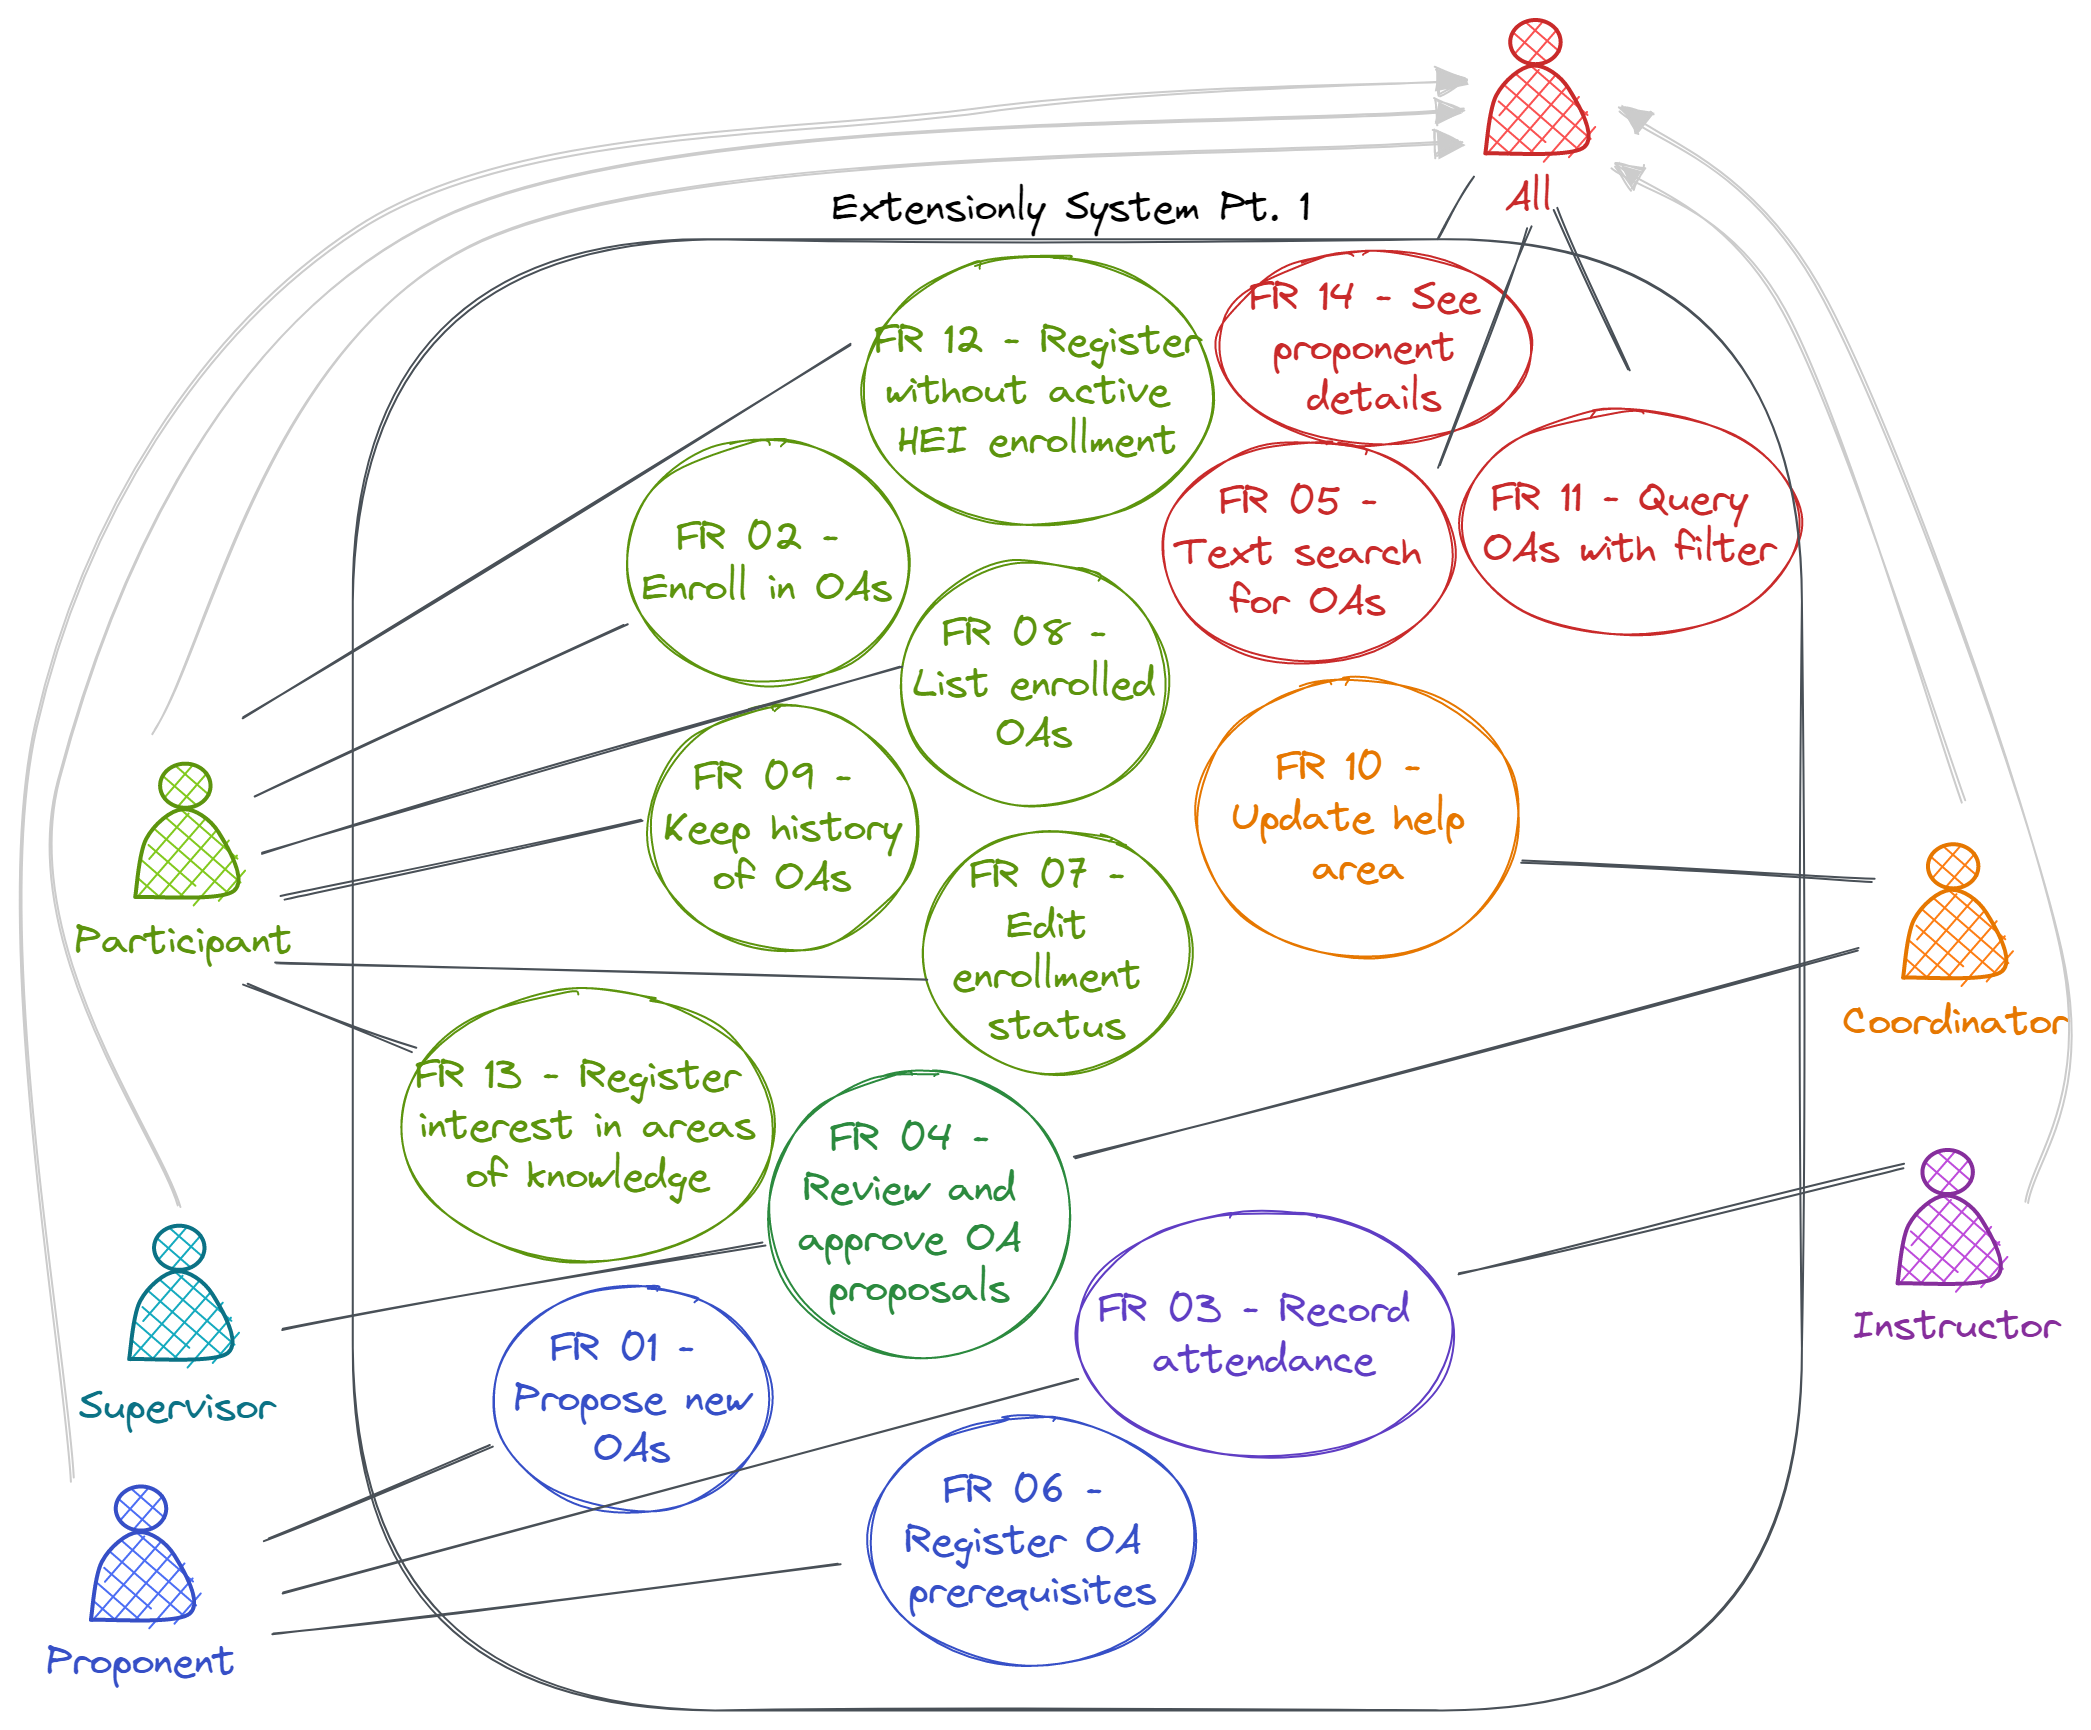
\includegraphics[width=15cm]{img/6-use-case-1.png}
  \end{center}
  \fonte{Author.}
\end{figure}

\begin{figure}[!htb]
  \caption{User Roles on the Last 8 \ac{FR}}\label{fig:use-case-2}
  \begin{center}
    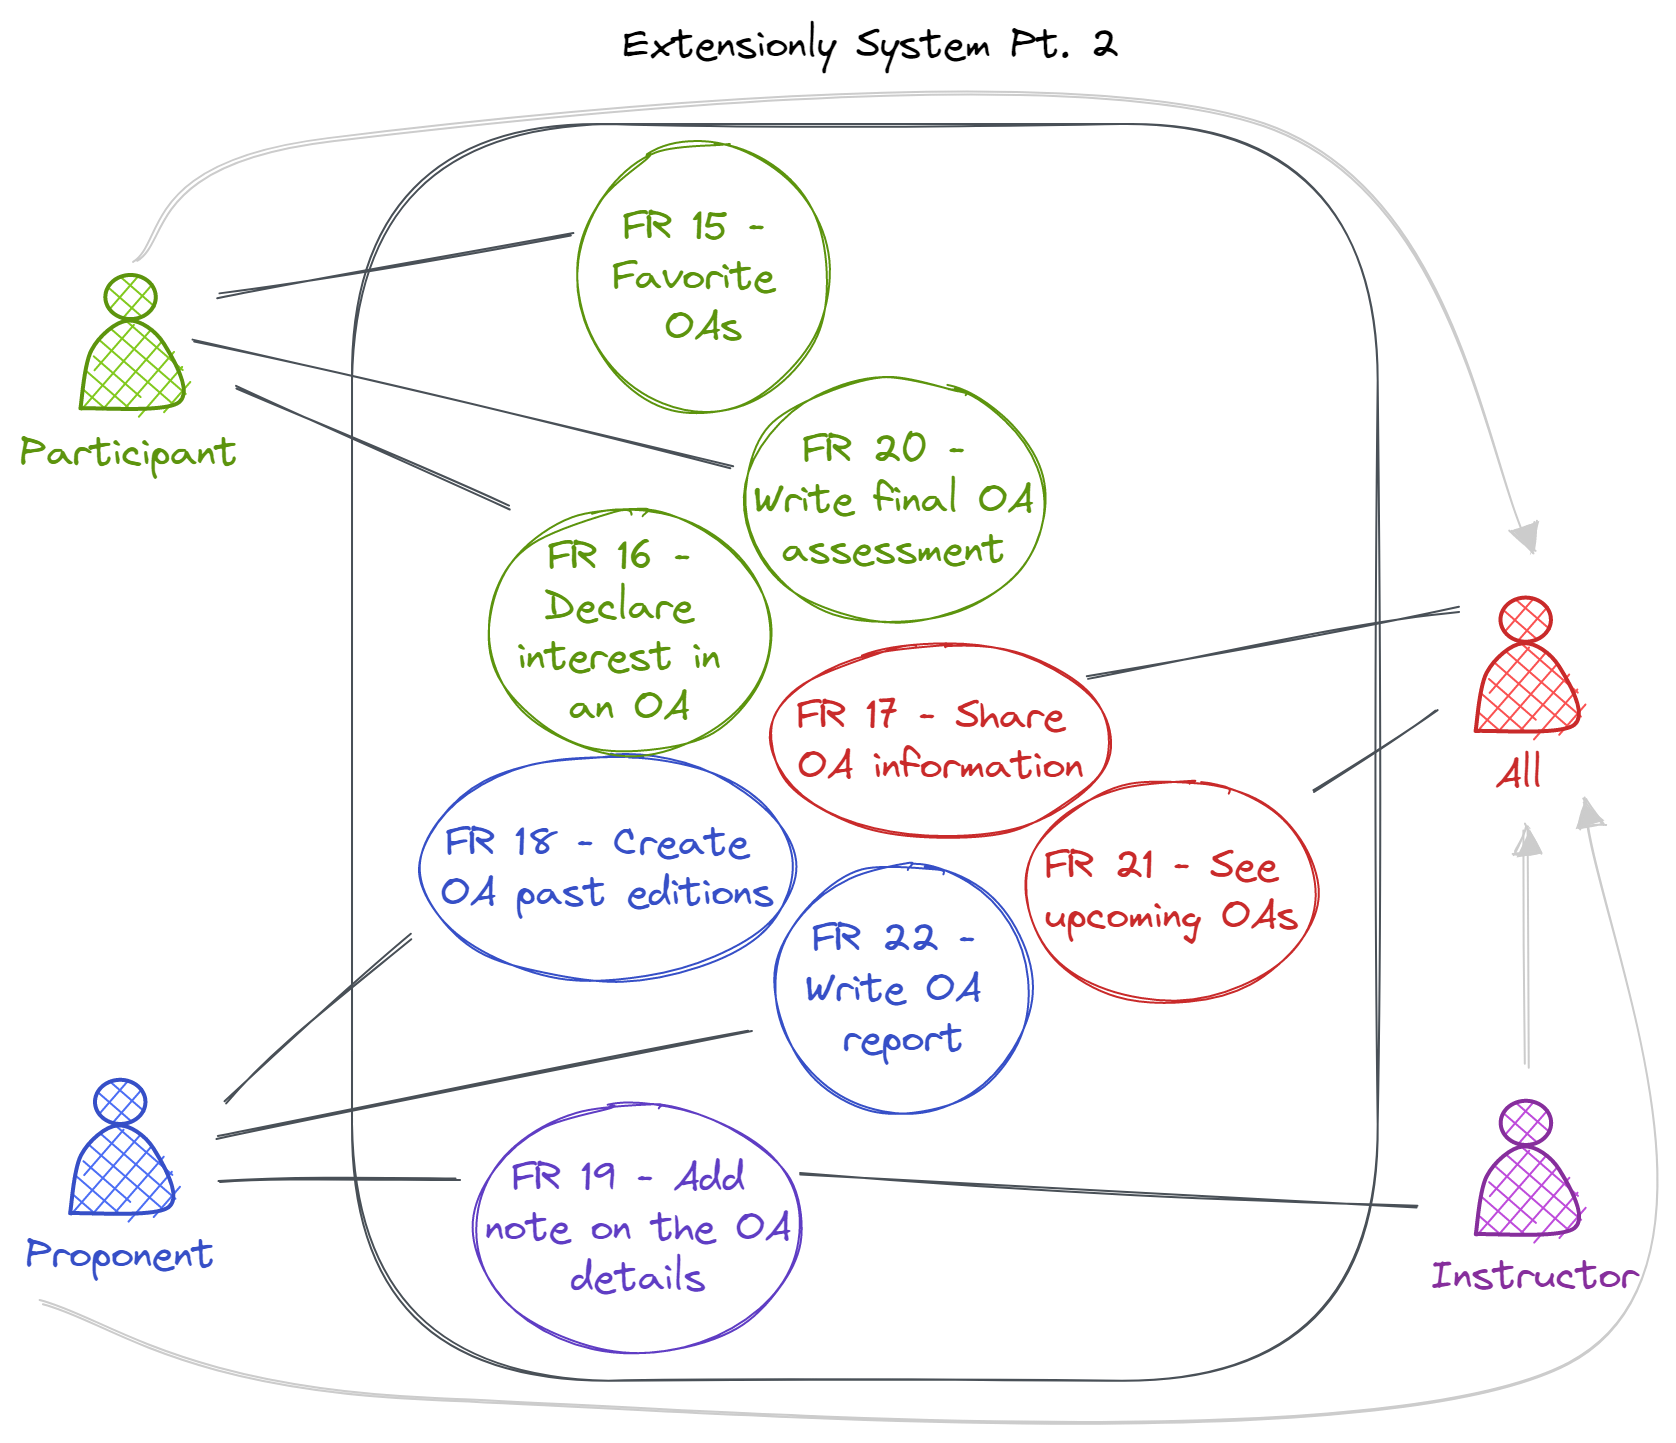
\includegraphics[width=12cm]{img/6-use-case-2.png}
  \end{center}
  \fonte{Author.}
\end{figure}

\subsection{User Stories Derived from the Requirements}
% ===================================
% Para o survey ser aplicado, um modelo de pergunta deveria ser montado com que a maioria dos respondentes compreendessem a mensagem a ser passada. 
% Para isso utilizando o modelo de historias de usuario que busca apresentar o papel do usuario, que vai desempenhar aquele determinado requisito, o objetivo da historia e o motivo por traz. 

For the survey to be applied, a question template should be set up so that most respondents understand the message to be conveyed. The user stories were derived from the \aclp{FR} presented by \Cref{tab:initial-requirements} and were divided between the roles of the system users. \Cref{tab:proponent-user-stories} shows user stories related to the proposer, then \cref{tab:instructor-user-stories} shows those related to the instructor, \Cref{tab:participant-user-stories} lists those related to the participant, and finally the \Cref{tab:coordinator-user-stories} contains the coordinator's user stories.

\begin{table}[!htb]
  \centering
  \setlength{\aboverulesep}{0pt}
  \setlength{\belowrulesep}{0pt}
  \caption{Proponent User Stories}
  \label{tab:proponent-user-stories}
  \footnotesize
  \begin{tabularx}{\textwidth}{c|X}
    \toprule
    \rowcolor[rgb]{0.753,0.753,0.753} \textbf{ID} & \textbf{User Story}                    \\
    \hline
    \rowcolor[rgb]{0.898,0.898,0.898} P1          & As a Proponent, I would like to propose an outreach activity, creating knowledge opportunities for other people.                                           \\
    P2                                            & As a Proponent, I would like to define desired prerequisites for enrollment in my outreach activity proposal, so that my applicants do not come unprepared.                                      \\
    \rowcolor[rgb]{0.898,0.898,0.898} P3          & As a Proponent, I would like my data to be shown along the details page of my outreach activity, so that participants have more details of who I am.                                \\
    P4                                            & As a Proponent, I would like to leave comments on the outreach activity page, to request some special material for carrying out the activity or just leave a note of mine for the participants.                              \\
    \rowcolor[rgb]{0.898,0.898,0.898} P5          & As a Proponent, I would like to fill in a general report on the progress of the outreach activity carried out, for archiving purposes.                                \\
    P6                                            & As a Proponent, I would like to register multiple editions of the same outreach activity, so that new participants can check past editions.                              \\
    \rowcolor[rgb]{0.898,0.898,0.898} P7          & As a Proponent or Instructor, I would like to get in touch with the participants of the outreach activity, so that it is easy to pass on information relevant to the activity.                                \\
    P8                                            & As a Proponent, I would like to receive the evaluation of the participants of my outreach activity in a detailed report/form format, so that I am aware of what I should improve for the next edition.                              \\
    \bottomrule
  \end{tabularx}
\end{table}
\begin{table}[!htb]
  \centering
  \setlength{\aboverulesep}{0pt}
  \setlength{\belowrulesep}{0pt}
  \caption{Instructor User Stories}
  \label{tab:instructor-user-stories}
  \footnotesize
  \begin{tabularx}{\textwidth}{c|X}
    \toprule
    \rowcolor[rgb]{0.753,0.753,0.753} \textbf{ID} & \textbf{User Story}         \\
    \hline
    \rowcolor[rgb]{0.898,0.898,0.898} I1          & As an Instructor, I would like to manage the attendance of registered participants so that certificates can be issued for those present.                                           \\
    \bottomrule
  \end{tabularx}
\end{table}
\begin{table}[!htb]
  \centering
  \setlength{\aboverulesep}{0pt}
  \setlength{\belowrulesep}{0pt}
  \caption{Participant User Stories}
  \label{tab:participant-user-stories}
  \footnotesize
  \begin{tabularx}{\textwidth}{c|X}
    \toprule
    \rowcolor[rgb]{0.753,0.753,0.753} \textbf{ID} & \textbf{User Story}                   \\
    \hline
    \rowcolor[rgb]{0.898,0.898,0.898} A1          & As a Participant, I would like to apply for outreach activities such as events, courses and lectures, to enter the waiting list and be accepted in the activity.                                          \\
    A2                                            & As a Participant, I would like to be able to search for outreach activities, so that I can find what I am looking for more easily.                                     \\
    \rowcolor[rgb]{0.898,0.898,0.898} A3          & As a Participant, I would like to cancel or edit the information of an outreach activity enrollment made by me, to have more freedom in case I change my mind.                                \\
    A4                                            & As a Participant, I would like to see previous editions of outreach activities, so that I can read past proposals.                              \\
    \rowcolor[rgb]{0.898,0.898,0.898} A5          & As a Participant, I would like to view the history of all the outreach activities I have participated in, so that I don't have to keep the record outside of the tool.                                \\
    A6                                            & As a Participant, I would like to have a help area within the system, to guide me with any questions or problems that I may face with the activity I signed up for.                              \\
    \rowcolor[rgb]{0.898,0.898,0.898} A7          & As a Participant without college enrollment, I would like to register in the system to participate in outreach activities that interest me.                                \\
    A8                                            & As a Participant, I would like to inform my interest in areas of knowledge, so that I can see outreach activities related to them.                              \\
    \rowcolor[rgb]{0.898,0.898,0.898} A9          & As a Participant, I would like to favor outreach activities that I deem interesting, so that I have easy access to them when I need them.                                \\
    A10                                           & As a Participant, I would like to show my interest in unavailable outreach activities, so that I will be notified when a new issue opens.                              \\
    \rowcolor[rgb]{0.898,0.898,0.898} A11         & As a Participant, I would like to register for outreach activities without registering in the system, so that my information is not saved.                                \\
    A12                                           & As a Participant, I would like to share information about the outreach activity, so that I can share it more easily with my friends.                              \\
    \rowcolor[rgb]{0.898,0.898,0.898} A13         & As a Participant, I would like to evaluate the outreach activity in which I participated, so that other participants can see the grade I assigned.                                \\
    A14                                           & As a Participant, I would like to see the outreach activities in which I am enrolled in the form of a calendar, so that I can organize myself better.                              \\
    \bottomrule
  \end{tabularx}
\end{table}
\begin{table}[!htb]
  \centering
  \setlength{\aboverulesep}{0pt}
  \setlength{\belowrulesep}{0pt}
  \caption{Coordinator User Stories}
  \label{tab:coordinator-user-stories}
  \footnotesize
  \begin{tabularx}{\textwidth}{c|X}
    \toprule
    \rowcolor[rgb]{0.753,0.753,0.753} \textbf{ID} & \textbf{User Story}         \\
    \hline
    \rowcolor[rgb]{0.898,0.898,0.898} C1          & As Coordinator, I would like to manage the submissions of new outreach activities carried out, so that each proposal goes through a review process before being accepted.                                           \\
    C2                                            & As Coordinator, I would like to issue certificates of participation with a certain number of hours for all involved, participants, instructors and coordinator, so that the individual's involvement in the outreach activity is proven.                                     \\
    \bottomrule
  \end{tabularx}
\end{table}
% ===================================

% ===================================
They were applyed directly, with no other refinements, in the final survey and can be seen in \Cref{appendix:questionnaire}.
However, in order to relate \acp{FR} with the questions and also update their ranking based on the survey results, \Cref{tab:stories-requirements-relation} was created.
% ===================================

\begin{table}[!htb]
  \centering
  \setlength{\aboverulesep}{0pt}
  \setlength{\belowrulesep}{0pt}
  \caption{Requirements vs User Stories Priorities}
  \label{tab:stories-requirements-relation}
  \footnotesize
  \begin{tabular}{c|c|c}
    \toprule
    \rowcolor[rgb]{0.753,0.753,0.753} \textbf{Requirement ID} & \textbf{Question/Story ID} & \textbf{Priority} \\
    \hline
    \rowcolor[rgb]{0.898,0.898,0.898} FR. 01                  & P1                         & Must have         \\
    FR. 02                                                    & A1                         & Must have         \\
    \rowcolor[rgb]{0.898,0.898,0.898} FR. 03                  & I1                         & Must have         \\
    FR. 04                                                    & C1                         & Must have         \\
    \rowcolor[rgb]{0.898,0.898,0.898} FR. 05                  & A2                         & Must have         \\
    FR. 06                                                    & P2                         & Should have       \\
    \rowcolor[rgb]{0.898,0.898,0.898} FR. 07                  & A3                         & Must have         \\
    FR. 08                                                    & A5                         & Must have         \\
    \rowcolor[rgb]{0.898,0.898,0.898} FR. 09                  & A5                         & Must have         \\
    FR. 10                                                    & A6                         & Must have         \\
    \rowcolor[rgb]{0.898,0.898,0.898} FR. 11                  & A2                         & Must have         \\
    FR. 12                                                    & A11                        & Will not have     \\
    \rowcolor[rgb]{0.898,0.898,0.898} FR. 13                  & A8                         & Must have         \\
    FR. 14                                                    & P3                         & Should have       \\
    \rowcolor[rgb]{0.898,0.898,0.898} FR. 15                  & A9                         & Must have         \\
    FR. 16                                                    & A10                        & Must have         \\
    \rowcolor[rgb]{0.898,0.898,0.898} FR. 17                  & A12                        & Should have       \\
    FR. 18                                                    & P6                         & Must have         \\
    \rowcolor[rgb]{0.898,0.898,0.898} FR. 19                  & P4                         & Should have       \\
    FR. 20                                                    & A13                        & Should have       \\
    \rowcolor[rgb]{0.898,0.898,0.898} FR. 21                  & A14                        & Must have         \\
    FR. 22                                                    & P5                         & Should have       \\
    \bottomrule
  \end{tabular}
\end{table}

\subsection{Roles}\label{ext:roles}
% ===================================
% Para o servico funcionar corretamente e de uma maneira organizada foram criados papeis de usuarios, controlando o que cada um pode ou não desempenhar dentro da ferramenta. 
% Estes papeis foram pensados tomando em conta os atuais papeis que existem relacionados a \acp{OA} dentro de uma \acp{HEI}, os papeissão os seguintes: 
% \begin{inparaenum}[(1)]
%   \item Participant - a listener, someone who enrolls to passively participate in the activity;
%   \item Instructor - a speaker, someone who presents or teaches something to participants;
%   \item Proponent - the one who proposes the \ac{OA}, usually a professor;
%   \item Coordinator - a role that can review and approve proposed activities for one campus;
%   \item Supervisor - usually does not interact with the process, but can monitor the system as a whole, having access to \ac{OA} in multiple campuses.
% \end{inparaenum}

For the service to work correctly and in an organized way, user roles were created, controlling what each one can or cannot perform within the tool.
These roles were designed taking into account the current roles that exist related to \acp{OA} within an \acp{HEI}, the roles are the following:
\begin{inparaenum}[(1)]
  \item Participant - a listener, someone who enrolls to passively participate in the activity;
  \item Instructor - a speaker, someone who presents or teaches something to participants;
  \item Proponent - the one who proposes the \ac{OA}, usually a professor;
  \item Coordinator - a role that can review and approve proposed activities for one campus;
  \item Supervisor - usually does not interact with the process, but can monitor the system as a whole, having access to \ac{OA} in multiple campuses.
\end{inparaenum}
% ===================================

% ===================================
% Além dos papeis citados acima, outro que não esta dentro do escopo do \ac{MVP} foi pensado, este é o ``External Participant'', que tem permissões semelhantes ao Participant, mas é uma pessoa que não tem relação direta com a universidade, mas que consegue se inscrever em atividades de extensão da mesma maneira.

In addition to the roles mentioned above, another that is not within the scope of \ac{MVP} was thought, this is the ``External Participant'', which has similar permissions to the Participant, but is a person who has no direct relationship with the university, but who manages to enroll in \aclp{OA} in the same way.
% ===================================
% Participant
% Instructor
% Proponent
% Coordinator
% Supervisor
% External

\section{Design Decisions}\label{sec:ext-design}
% ===================================
This section describes the design decisions taken to carry out this study and the development of this tool:
\begin{description}
    % \item[\textbf{Programming Language:}] \ac{TS} foi escolhido porque ela fornece diversas soluções e frameworks disponiveis para uso, que simplificam o desenvolvimento. Um ponto positivo e que se destaca da linguagem base \ac{JS}, é que esta linguagem adiciona tipagem estática ao código, reduzindo muito as chances de erro por sintaxe e agilizando o desenvolvimento. Outro fator de escolha se da pela experiencia dos desenvolvedores, que ja estão familiarizados com esta linguagem e seus frameworks, a mesma linguagem foi escolhida no frontend, facilitando o entendimento entre os códigos fonte.  
    
    \item[\textbf{Programming Language:}] \ac{TS} was chosen because it enriches \ac{JS} with a module system, classes, interfaces, and a static type system, as said by \textcite{Bierman_2014}.
    The authors also comments that a typed language helps a lot in development, finding and preventing bugs, providing auto-completion, hover tips, navigation through the code, and also helps in code refactoring.
    % A positive point that stands out from the base language \ac{JS} is that this language adds static typing to the code, greatly reducing the chances of syntax errors and speeding up development. 
    Another choice factor is given by the experience of the developers, who are already familiar with this language and its frameworks, the same language was chosen in the frontend, facilitating the understanding between the source codes;
    % ===================================
    
    % ===================================
    % \item[\textbf{Framework:}] NestJS desenvolvido por \cite{nestDocs}, foi o framework escolhido devido o seu potencial e facilidade em escalabilidade de aplicações. Ele possui uma organizaçao de arquivos muito simples, chamada de model-service-controller, onde a camada model é responsavel pelo gerenciamento de dados, controller é responsável pelo gerenciamento de entradas e saidas de requisiçoes na nossa aplicaçao e a camada service contém toda a lógicade implementação, parte dessa organizaçao pode ser vista na \Cref{fig:architecture}.
    
    \item[\textbf{Framework:}] NestJS developed by \textcite{nestDocs}, was the chosen framework due to its potential and ease of application scalability. The author also mention that it has a very simple file organization, called model-service-controller, where the model layer is responsible for managing data, controller is responsible for managing input and output requests in our application and the service layer contains all the logic of implementation, part of this organization can be seen in \Cref{fig:architecture};
    % ===================================
    
    % ===================================
    % Outro ponto muito forte do NestJS é o seu suporte a modularização, em que mesmo que o código seja escrito de uma maneira monolítica, as controllers e servicos estarão separadas por responsabilidades, facilitando uma possivel futura transição entre arquiteturas. Combinado a modularizaçao, este framework fornece um poderoso sistema de injeção de dependencias permitindo que códigos sejam reutilizados entre módulos de maneira muito simples, basta injeta-lo no modulo destino.
    
    Another very strong point of NestJS is its support for modularization, as demonstrated by \textcite{nestDocs},  in which even if the code is written in a monolithic way, the controllers and services will be separated by responsibilities, facilitating a possible future transition between architectures. Combined with modularization, this framework provides a powerful dependency injection system allowing code to be reused between modules in a very simple way, just inject it into the target module;
    % ===================================
    
    % ===================================
    % Em relaçao a persistencia de dados, o NestJS permite a utilização de \acp{ORM}, que facilitam esta interaçao com os bancos de dados, ficando ele responsavel por todas as complicaçoes envolvidas neste processo, mais sobre o assunto sera explicado no \Cref{data-persistance}.
    
    Regarding data persistence, Nest allows the use of \acp{ORM}, which are, as \textcite{Wiphusitphunpol_2017} said, a tool for mapping database query results to strongly typed or weakly typed objects in object-oriented programming languages, increasing the speed of development and maintainability. More on the subject will be explained in \Cref{data-persistence};
    % ===================================
    
    % ===================================
    % \item[\textbf{Architecture:}] A arquitetura escolhida para o desenvolvimento da Extensionly foi server-client model que de acordo com \textcite{puliafito_riccobene_scarpa}, é uma arquitetura que dispõe servicos ou servidores duplicados para uma rede de clientes que os utilizam. 
    
    \item[\textbf{Architecture:}] The architecture chosen for the development of Extensionly was the server-client model which, according to \textcite{puliafito_riccobene_scarpa}, is an architecture that has duplicated services or servers for a network of clients that use them.
    % ===================================
    
    % ===================================
    % Na \Cref{fig:architecture} está representado a arquitetura pensada para este \ac{MVP}, ainda há possibilidades de melhoria como por exemplo, adicionar um Load Balancer entre as chamadas do cliente para o servidor, sendo responsável por duplicar as instâncias existentes do servidor caso haja um pico de acessos na aplicação. Outra melhoria está na adição de cache nas chamadas para o banco de dados, que serve para acessar mais rapidamente dados que estão sendo requisitados com frequencia.
    
    The architecture designed for this \ac{MVP} is represented in \Cref{fig:architecture}, there are still possibilities for improvement, such as adding a server load balancer between client calls to the server, being responsible for spreading out the transmission of information flow and data operations, as well as lowering the risk of information loss and computing time, as \textcite{Chen_2015} described.
    Another improvement is the addition of caching in calls to the database, which serves to more quickly access data that is being requested frequentl.
    % ===================================
    
    \begin{figure}[htb]
      \caption{Backend Achitecture}\label{fig:architecture}
      \begin{center}
        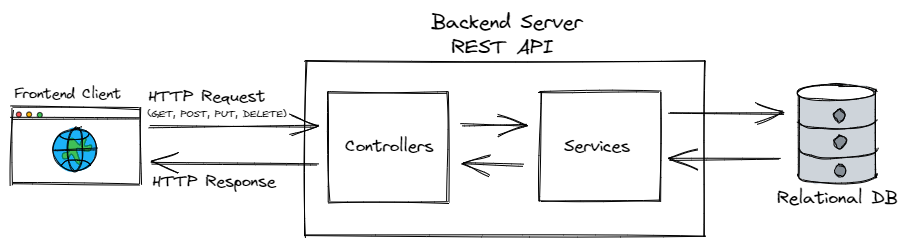
\includegraphics[width=15cm]{img/6-architecture.png}
      \end{center}
      \fonte{Author.}
    \end{figure}
    
    % ===================================
    % O servidor backend utiliza a arquitetura API Rest, onde \ac{API}, de acordo com \textcite{restApi}, utiliza de requisições \ac{HTTP} como: 
    % \begin{inparaenum}[(1)]
    %   \item GET;
    %   \item POST;
    %   \item PUT;
    %   \item DELETE, 
    % \end{inparaenum} para realizar a manipulaçao de dados do sistema. Em seguida, o autor define \ac{REST} como restrições utilizadas para que as requisições \ac{HTTP} atendam as diretrizes definidas na arquitetura, dentre elas estão:
    % \begin{inparaenum}[(1)]
    %   \item Utilizar arquitetura cliente-servidor;
    %   \item Não possuir estado, requisiçoes sendo independentes;
    %   \item Possuir cache;
    %   \item Possuir uma nterface uniforme.
    % \end{inparaenum}
    
    The backend server uses the REST API architecture, where \ac{API}, according to \textcite{restApi}, uses \ac{HTTP} requests such as:
    \begin{inparaenum}[(1)]
      \item GET;
      \item POST;
      \item PUT;
      \item DELETE, 
    \end{inparaenum} to perform system data manipulation. Then, \textcite{restApi} defines \ac{REST} as restrictions used so that \ac{HTTP} requests meet the guidelines defined in the architecture, among them are:
    \begin{inparaenum}[(1)]
      \item Use server-client architecture;
      \item Not having state, requests being independent;
      \item Have cache;
      \item Have a uniform interface;
    \end{inparaenum}
    % ===================================
    
    % Client Server
    % API
    % Diretrizes REST
    % ===================================
    % \item[\textbf{License:}] A ferramenta Extensionly sera em um primeiro momento uma soluçao Open Source, ja que desta maneira outras pessoas poderão contribuir com a aplicação. Entretanto existe a possíbilidade de que a aplicaçao seja fornecida em modelo de serviço no futuro, logo funcionalidades pagas podem ser adicionadas.
    
    \item[\textbf{License:}] The Extensionly backend is licensed under the GNU General Public License v3.0, which is an open source license and is very permissive, allowing even for commercial use. However, it is very important to keep in mind that all works and modifications must be released under the same license, with the source code made available, and that the distribution of closed source versions is not permitted. Additionally, it does not provide the software with any guarantees or liabilities \cite{gnugpl3}.
    
    % ===================================
    % Open-source
    % Futuramente Pago algumas funcionalidades
    % ===================================
    % \item[\textbf{Data Persistence:}]\label{data-persistance}
    % Para realizar a persistencia dos dados, será utilizado banco de dados relacional, que é o mais adequado ao carater do problema por ter muitas relaçoes entre os objetos presentes no sistema, para isso será utilizado o \ac{DBMS} \ac{MySQL}.
    \item[\textbf{Data Persistence:}]\label{data-persistence} To perform the data persistence, a relational database will be used, which is the most suitable for this problem because it has many relationships between the objects present in the system, for which \ac{DBMS} \ac{MySQL} will be used.
    % ===================================
    
    % ===================================
    % Também sera utilizado o Prisma como o \ac{ORM} da ferramenta, que de acordo com \textcite{prisma}, is an \ac{ORM} that helps app developers build faster and make fewer errors, disponibilizando um schema do banco de dados que allows developers to define their application models in an intuitive data modeling language, reducing boilerplate so developers can focus on the important parts of the app.
    
    Prisma will also be used as the \ac{ORM} of the tool, which according to \textcite{prisma}, is an \ac{ORM} that helps app developers build faster and make fewer errors, providing a database schema which allows developers to define their application models in an intuitive data modeling language, reducing boilerplate so developers can focus on the important parts of the app;
    % ===================================
    % Banco relacional
    % MySQL
    % Prisma
    % ===================================
    % \item[\textbf{DevOps:}] Para que a aplicação seja automatica quando se trata de build, testes e deploy, serão utilizadas algumas soluçoes de DevOps, comecando com as pipelines do GitHub Actions, que são muito simples para o entendimento e ja estão alocadas junto com o repositório\footnote{Extensionly Backend code is available at \url{https://github.com/IgorDalepiane/extensionly-backend-service}} do backend. 
    % Com as pipelines é possível bloquear um \ac{PR} até que o código para ser adicionado esteja de acordo com as diretrizes definidas, realizar o deploy quando determinadas açoes acontecem, testar codigo automaticamente, tudo isso melhora o controle e organizaçao do código, será utilizado como base o tutorial\footnote{CICD Tutorial is available at \url{https://github.com/IgorDalepiane/CICD-Tutorial/wiki}} feito pelo autor.
    
    
\end{description}

\section{\ac{DevOps}}\label{sec:dev-ops}

\textcite{perera2017improve} describes \ac{DevOps} as a set of techniques that allows developers and operators to interact and work together to provide software and services quickly, consistently, and of higher quality. The solution chosen was the GitHub Actions, which are very simple to understand and already are allocated along with the backend repository.

% ========================================================
% Integrado a prática de DevOps o autor \textcite{Shahin_2017} explica três diferentes termos muito importantes para o entendimento do funcionamento desta prática, a estrutura da pipeline e do funcionamento na prática destes termos esta representada na \Cref{fig:relationship-ci-cde-cd}, os termos são os que seguem:

Integrated into the \ac{DevOps} practice, the author \textcite{Shahin_2017} explains three different terms that are very important to understand how this practice works, the structure of the pipeline and how these terms work in practice is represented in \Cref{fig:relationship-ci-cde-cd}, the terms are as follows:
% ========================================================

\begin{description}
    % ========================================================
    % \item[\textbf{\ac{CI}}] A definiçao do termo diz a respeito de times de desenvolvimento mergearem trabalho de desenvolvimento com mais frequencia, aumentando a qualidade do produto, o desempenho do time e reduzindo prazos de entrega, incluindo passos de build e testes automatizados.
    
    \item[\textbf{\ac{CI}}] The definition of the term is about development teams merging development work more frequently, increasing product quality, team performance and reducing delivery times, including steps of build and automated tests.
    
    % ========================================================
    % \item[\textbf{\ac{CDE}}] Este termo representa o processo que garante que a aplicação vai sempre estar em um estado pronto para ser enviada para produçao, passando em pipelines com testes automatizados e checagens de qualidade. Esta prática reduz o esforço necessário e riscos envolvidos na hora de enviar um software para produçao.
    
    \item[\textbf{\ac{CDE}}] This term represents the process that guarantees that the application will always be in a state ready to be sent to production, passing through pipelines with automated tests and quality checks. This practice reduces the effort required and risks involved when sending software to production.
    % ========================================================
    % \item[\textbf{\ac{CD}}] Este termo pode ser muito semelhante ao anterior, pois busca fazer as mesmas coisas mas de uma maneira mais automatica, enquanto o item anterior necessita da ação humana para aprovar um deploy para produçao, este termo utiliza de pipelines que enviam diretamente qualquer mudança de código mergeada, para o ambiente real de produção.
    
    \item[\textbf{\ac{CD}}] This term can be very similar to the previous one, as it seeks to do the same things but in a more automatic way, while the previous item needs human action to approve a deploy for production, this term uses pipelines that send any merged code changes directly to the real production environment.
    % ========================================================
\end{description} 

\begin{figure}[htb]
  \caption{The relationship between continuous integration, delivery and deployment}\label{fig:relationship-ci-cde-cd}
  \begin{center}
    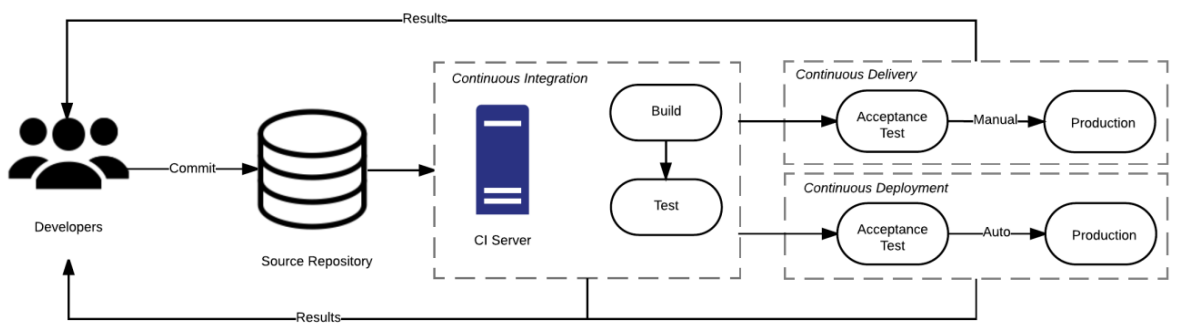
\includegraphics[width=15cm]{img/6-ci-cde-structure.png}
  \end{center}
  \fonte{\cite{Shahin_2017}.}
\end{figure}
% ========================================================
% Os termos que serão implementados no backend da ferramenta Extensionly serão o \ac{CI} e o \ac{CDE}, pois assim é possivel ter mais controle no versionamento da solução, e sempre mantendo ela testada e pronta para ser enviada para produçao.

The terms that will be implemented in the backend of the Extensionly tool will be \ac{CI} and \ac{CDE}, because this way it is possible to have more control in the versioning of the solution, and always keeping it tested and ready to be sent to production.
% ========================================================
% Para que a aplicaçao de DevOps funcione corretamente uma boa configuraçao de repositório, projetos, deploys e pipelines deve ser executada, para isso sera utilizado o tutorial\footnote{CICD Tutorial is available at \url{https://github.com/IgorDalepiane/CICD-Tutorial/wiki}} desenvolvido pelo autor deste \ac{TP}.

For the \ac{DevOps} application to work correctly, a good configuration of repository, projects, deploys and pipelines must be performed, for this will be used the tutorial\footnote{CICD Tutorial is available at \url{https://github.com/IgorDalepiane /CICD-Tutorial/wiki}} developed by the author of this \ac{TP}.
% ========================================================

% With pipelines it is possible to block a \ac{PR} until the code to be added complies with the defined guidelines, perform the deployment when certain actions happen, test code automatically, all this improves the control and organization of the code, it will be used as a basis the tutorial\footnote{CICD Tutorial is available at \url{https://github.com/IgorDalepiane/CICD-Tutorial/wiki}} made by the author.
% ===================================
% ===================================
% Para a realizaçao do deploy, será utilizado o Hiroku, que é uma solução gratis e muito eficaz, sendo o suficiente para o proposito deste \ac{MVP}.

For the deployment, Heroku will be used, which according to \textcite{heroku} is a cloud platform that lets developers build, deliver, monitor and scale apps. Heroku's \ac{PaaS} service will be used, which according to \textcite{Zvarevashe2014TheAO}, is a service that allows the contractor to publish their applications in the cloud without having to install any software on their local machine, it also already solves configurations related to infrastructure and machine configurations, allowing the developer to focus only on the development of the tool.
% ===================================
% Pipelines, testes, build
% Deploy, Netlify, Vercel ou Hiroku

\section{Chapter Summary}
% ===================================
% Este capitulo discorreu sobre decisões relacionadas a produção da ferramenta Extensionly, primeiro sendo explicado alguns pontos de atenção na \Cref{sec:ext-considerations}, logo na \Cref{sec:ext-req}, foram apresentados os requisitos finais levantados pela literatura cinza e as estorias de usuario com as suas pontuaçoes recebidas pela execução do survey. Por fim, \Cref{sec:ext-design} reporta as decisoes de design para a execução do projeto, como tecnologias e arquitetura utilizada.

This chapter discussed decisions related to the production of the Extensionly tool, first explaining some points of attention in \Cref{sec:ext-considerations}, then in \Cref{sec:ext-req}, the final requirements raised by grey literature review and user stories with their scores received for carrying out the survey, are shown. \Cref{sec:ext-design} reports the design decisions for the execution of the project, such as technologies and architecture used. Finally, in \Cref{sec:dev-ops}, some terms related to \ac{DevOps} were discussed, along with the choices that will be used in the tool development processes.

% ===================================


% \section{Requirement Engineering}
% \subsection{Requirements Elicitation, Modeling and Analysis}
% \subsection{User Stories}

% \section{Features}
% \begin{landscape}
\begin{figure}[!htb]
\caption{Taxonomy of performance testing tools represented by feature model.}
\label{fig:featuremodel}
\begin{adjustbox}{max width=1.5\textwidth}
%% https://tex.stackexchange.com/questions/335708/feature-diagram-in-latex
    \begin{forest}  
    disjunction tree,
    disjuncts from'=1,
    concrete from'=1,
    concrete colour=blue!55!cyan!40,
    abstract colour=blue!85!cyan!15,
    draw colour=darkgray,
    [Performance Testing Process
        [Profiles/Roles, mandatory, l=25mm
            [Performance Engineer, l=20mm
                [Architect, l=20mm]
                [Tester, l=20mm]
                [Analyst, l=20mm]
            ]
        ]
        [Methods, mandatory, l=25mm
            [Scripting, l=20mm]
            [CR, l=20mm]
            [MBT, l=20mm]
        ]
        [Artifacts, mandatory, l=25mm
            [Test Plan, optional, l=20mm]
            [Model, optional, l=20mm]
            [Script, l=20mm]
            [Workload, l=20mm]
            [Scenario, l=20mm]
            [Test Report, l=20mm]
        ]
        [Approaches, mandatory, l=25mm,
            [Load, l=20mm]
            [Stress, l=20mm]
            [Endurance, l=20mm]
            [Spike, l=20mm]
        ]
        [Stages, mandatory, l=71mm
            [Pre-Test, mandatory, l=20mm
                [Planning, optional, l=20mm]
                [Scripting, l=20mm]
                [Design, l=20mm]
                [Configuration, l=20mm]
            ]
            [Test, mandatory, l=20mm
                [Execution, l=20mm]
                [Monitoring, l=20mm]
            ]
            [Post-Test, mandatory, l=20mm
                [Analysis, optional, l=20mm]
                [Reporting, l=20mm]
            ]
        ]
    ]
    \end{forest}
    \end{adjustbox}
    \centering
    \fonte{Author.}
    \end{figure}
\end{landscape}
% \subsection{Roles}

% \section{Development}
% \subsection{Technology Stack}
% \subsection{Programming Paradigm}
% \subsection{Design Patterns}

% \section{Software Architecture}
% \subsection{DevOps}
% \subsection{Pipeline}

% \section{Testing}

% \section{Software Artifacts}
% \subsection{Domain Model}
% \subsection{Component Diagram}
% \subsection{Database Schema}
